\documentclass[11pt]{article}

% ---------- packages ----------
\usepackage[utf8]{inputenc}
\usepackage[T1]{fontenc}
\usepackage{lmodern}
\usepackage[a4paper,margin=1in]{geometry}
\usepackage{amsmath,amssymb,amsthm}
\usepackage{xcolor}
\usepackage[most]{tcolorbox}
\usepackage{booktabs}
\usepackage{array}
\usepackage{enumitem}
\usepackage{titlesec}
\usepackage{parskip}
\usepackage{graphicx}
\usepackage{tikz}
\usetikzlibrary{arrows.meta,positioning,fit,backgrounds,calc}
\usepackage[colorlinks=true,linkcolor=blue!55!black,urlcolor=blue!55!black,citecolor=blue!55!black]{hyperref}

% ---------- colors ----------
\definecolor{accent}{HTML}{00695C}
\definecolor{accent2}{HTML}{2E7D32}
\definecolor{accent3}{HTML}{B23A00}
\definecolor{softgray}{HTML}{F2F4F7}
\definecolor{coolc}{HTML}{E3F2EF}
\definecolor{warmc}{HTML}{FFF3E0}
\definecolor{hotc}{HTML}{FDE7E9}

% ---------- section styling ----------
\titleformat{\section}{\Large\bfseries\color{accent}}{\thesection}{0.6em}{}
\titleformat{\subsection}{\large\bfseries\color{accent!85!black}}{\thesubsection}{0.6em}{}
\titlespacing*{\section}{0pt}{1.5em}{0.6em}

% ---------- boxes ----------
\newtcolorbox{motivebox}[1][]{
  colback=coolc, colframe=accent, boxrule=0.6pt, arc=2pt,
  left=8pt,right=8pt,top=5pt,bottom=5pt,
  fonttitle=\bfseries, title={Motivation in one paragraph}, #1}
\newtcolorbox{theorybox}[1][]{
  colback=green!5, colframe=accent2, boxrule=0.6pt, arc=2pt,
  left=8pt,right=8pt,top=5pt,bottom=5pt,
  fonttitle=\bfseries, title={Theory target}, #1}
\newtcolorbox{claimbox}[1][]{
  colback=accent3!8, colframe=accent3, boxrule=0.8pt, arc=2pt,
  left=8pt,right=8pt,top=6pt,bottom=6pt,
  fonttitle=\bfseries, title={Defensible paper claim}, #1}
\newtcolorbox{riskbox}[1][]{
  colback=red!4, colframe=red!55!black, boxrule=0.6pt, arc=2pt,
  left=8pt,right=8pt,top=5pt,bottom=5pt,
  fonttitle=\bfseries, title={Main risk \& mitigation}, #1}

\newtheorem{claim}{Target Theorem}

\newcommand{\term}[1]{\textbf{\color{accent!85!black}#1}}
\newcommand{\R}{\mathbb{R}}
\newcommand{\E}{\mathbb{E}}
\newcommand{\norm}[1]{\lVert #1 \rVert}
\newcommand{\Prob}{\mathbb{P}}

\begin{document}

% ---------------- TITLE ----------------
\begin{titlepage}
\centering
\vspace*{1.6cm}
{\Huge\bfseries\color{accent} Shufflerless-CI\par}
\vspace{0.4cm}
{\Large\bfseries\color{accent} RoPE-Safe Latent--Residual KV for\\ Stationary Collaborative Decoding\par}
\vspace{0.5cm}
{\large No large tensor crosses the CPU--GPU (or device) boundary\\ during steady-state decoding\par}
\vspace{1.4cm}
\begin{tcolorbox}[colback=accent3!8,colframe=accent3,width=0.92\textwidth,arc=3pt]
\centering\bfseries
Shufflerless-CI converts the memory wall from an unpredictable runtime swapping problem into
an explicitly budgeted representation-and-placement problem. A fixed, RoPE-safe projection
creates the low-rank KV bulk; only small input-dependent innovations are compressed online.
The cache remains stationary and attention never materializes the full old KV.
\end{tcolorbox}
\vspace{1.0cm}
\begin{tcolorbox}[colback=softgray,colframe=accent,width=0.92\textwidth,arc=3pt]
\centering
This July 2026 revision separates \emph{what} is compressed from \emph{when}: a
weight-side, offline latent projection handles the stable bulk, while a block-wise online
sparse residual preserves prompt-specific outliers. It then co-optimizes that representation
with the layer partition and memory reserve on the FSU poster's cluster.
\end{tcolorbox}
\vfill
{\normalsize Research proposal \;\textbullet\; \today\par}
\end{titlepage}

\tableofcontents
\newpage

% ================================================================
\section{Why this idea, among the six}
\label{sec:select}

Six directions were considered. The earlier draft treated compressed-domain attention as the
novel core. That is no longer defensible: Eigen Attention~\cite{eigenattention} already
computes in a low-rank space, Palu~\cite{palu} creates latent KV from factorized projections,
and RAP~\cite{rap} removes RoPE-induced reconstruction for aligned projections. The revised
paper is a \term{new systems setting and co-design}: a RoPE-safe latent cache plus sparse
prompt-specific innovations, jointly budgeted with heterogeneous pipeline placement to keep
each layer and its cache stationary.

\begin{center}
\renewcommand{\arraystretch}{1.28}
\small
\begin{tabular}{@{}p{4.5cm}ccc p{4.0cm}@{}}
\toprule
\textbf{Candidate} & \textbf{Nov.} & \textbf{Feas.} & \textbf{Pub.} & \textbf{Verdict} \\
\midrule
\textbf{1. Latent--residual Shufflerless-CI} & Med--High & High & High & \textbf{Selected} (flagship) \\
2. Compute-at-the-cache (exact distributed softmax) & Low--Med & High & Med & Local hot/cold merge only \\
3. Predictive sparse KV prefetch & Low--Med & High & Med & Complementary; near ScoutAttention \\
4. Session-specialized weight residency & Med & Med & Med--High & Strong but separate (weights, not KV) \\
5. Risk-aware repartitioning & Low--Med & High & Med--High & \emph{Merged in} as the no-shuffle planner \\
6. Compute/load/fetch/skip controller & Med & Med & Med & \emph{Merged in} lightly as the adaptive controller \\
\bottomrule
\end{tabular}
\end{center}

\noindent The selected project deliberately borrows its compression primitives and claims
novelty at their \emph{coupling}: (i) fixed RoPE-safe latent birth, (ii) sparse residuals
created once when a hot block ages, and (iii) a stage planner that allocates rank and residual
bytes where they reduce the pipeline bottleneck. Remote KV sharding and reinforcement learning
are removed from the first paper because they add network round trips and scope without helping
the main performance claim.

% ================================================================
\section{Motivation}

\begin{motivebox}
On-device and edge LLM decoding hits the \term{memory wall}: model weights plus a KV cache
that \emph{grows every token} cannot all stay in the memory budget assigned to an accelerator
stage. Reactive paging~\cite{pagedattention} then creates transfers, synchronization, and tail
latency. Pure activation-side compression is not the answer: running an SVD as the cache grows
can cost more than the attention it saves. The research question is therefore: \emph{can the
KV be born small, corrected cheaply for each prompt, and co-placed with its owning layers so
that steady-state decoding has no large cache transfers or reconstruction buffers?}
\end{motivebox}

\subsection{The three failure modes of compression-alone}
Any scheme that merely stores KV compactly can still incur:
\begin{enumerate}[leftmargin=1.5em,itemsep=1pt]
\item \term{Load:} the compressed data is fetched from CPU when needed;
\item \term{Reconstruct:} the dense KV tensor is rebuilt on the GPU before attention;
\item \term{Buffer bloat:} temporary reconstruction buffers consume the saved memory.
\end{enumerate}
Shufflerless-CI removes all three by (i) generating the low-rank bulk through fixed projection
factors, not runtime decomposition; (ii) adding only a sparse block-wise residual when an exact
hot block ages; and (iii) keeping every layer and its KV on one owner stage. On Jetson's unified
memory, ``shuffle'' includes explicit copies, page migration, and synchronization; all must be
measured rather than inferred from allocation APIs.

% ================================================================
\section{Background and related work}

\subsection{The FSU pipelined-inference poster (the base system)}
The poster's \term{CI-Inf}~\cite{poster} partitions a decoder by layers across heterogeneous
Jetson devices; each device holds whole layers and keeps its layers' KV cache resident,
avoiding CPU$\leftrightarrow$GPU swapping and cutting per-token latency 40\%
(325$\to$192\,ms). Shufflerless-CI extends CI-Inf so that residency is \emph{guaranteed up to a
budgeted context length}, via a latent--residual cache and joint stage placement.
Placement/parallelism machinery is inherited from HexGen~\cite{hexgen} and
Jupiter~\cite{jupiter}; fairness across devices from FOCI~\cite{foci}.

\subsection{KV-cache compression --- and the novelty boundary}
Low-rank, sparse, and hybrid KV compression are active research, so none is by itself novel:
\begin{itemize}[leftmargin=1.5em,itemsep=1pt]
\item \term{ShadowKV}~\cite{shadowkv}: low-rank keys kept on GPU, values \emph{offloaded to CPU}
and loaded back on demand.
\item \term{Lexico}~\cite{lexico}: sparse coding over a universal dictionary; KV is
\emph{reconstructed} from atoms before use.
\item \term{GEAR}~\cite{gear}: quantization $+$ a low-rank term for quantization error $+$ a
sparse term for outliers --- literally low-rank$+$sparse, but reconstructed.
\item \term{RocketKV}~\cite{rocketkv}: two-stage eviction $+$ hybrid top-$k$ sparse attention
(single device).
\item \term{Eigen Attention}~\cite{eigenattention}: performs attention directly in a
low-rank space; \term{RAP}~\cite{rap} uses RoPE-aligned pruning to avoid reconstruction.
\item \term{OjaKV}~\cite{ojakv}: combines exact anchors with an online-adapted low-rank
subspace; \term{STAR-KV}~\cite{starkv} performs fine-grained adaptive rank control; and
\term{LCA}~\cite{lca} condenses context directly inside an MLA latent space.
\end{itemize}
The defensible gap is narrower: existing cache methods optimize a single model/device cache;
CI-Inf fixes the layer split. This project jointly chooses the RoPE-safe projection, sparse
innovation budget, exact hot window, and heterogeneous layer partition under an explicit
no-shuffle constraint. This is a \emph{novelty hypothesis}, not a settled fact; the literature
audit must be refreshed immediately before submission.

\subsection{Collaborative / distributed attention (the aggregation primitive)}
The exact-merge machinery Shufflerless-CI uses is grounded in \term{online-softmax}
computation~\cite{onlinesoftmax} and \term{FlashAttention}~\cite{flashattention}, which compute
attention block by block via running max, sum, and output statistics.
\term{Ring Attention}~\cite{ringattention} distributes those blocks across devices but moves
KV blocks. \term{CAKE}~\cite{cake} chooses whether to compute or load KV;
\term{ScoutAttention}~\cite{scoutattention} performs GPU--CPU collaborative block-sparse
attention. Shufflerless-CI instead treats remote per-layer attention as an emergency fallback:
the fast path keeps the cache local to its layer owner and uses online-softmax only to merge
local exact-hot and compressed-old blocks.

\subsection{Tensor foundations}
The low-rank$+$sparse model is Robust PCA~\cite{rpca}; factorizations are CP/Tucker~\cite{kolda}
and Tensor-Train~\cite{tt}; low-rank$+$sparse weight structure is LoSparse~\cite{losparse};
attention low-rankness is Linformer~\cite{linformer}; heavy-hitter token sparsity is
H2O~\cite{h2o}; low-rank KV projection precedents include Palu~\cite{palu}, Eigen
Attention~\cite{eigenattention}, and MLA~\cite{deepseekv2}.

% ================================================================
\section{Method}
\label{sec:method}

\subsection{The stationarity principle and per-stage memory layout}
Each pipeline stage \emph{permanently} stores its weights, an exact GPU-resident window of the
$W$ most recent KV entries, a compressed representation of older KV, and enough workspace that
decoding never triggers emergency swapping:

\begin{center}
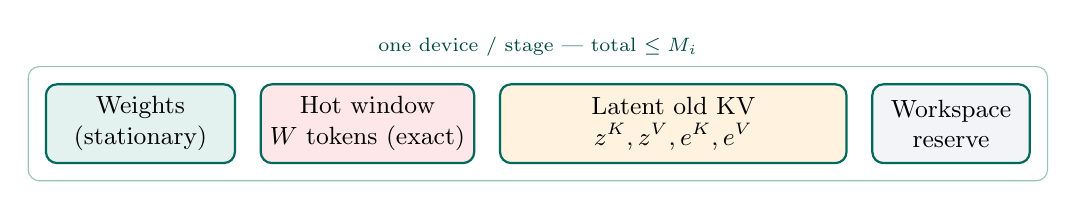
\begin{tikzpicture}[
  blk/.style={draw=accent, rounded corners, minimum height=1.0cm, align=center, thick, font=\small},
  ar/.style={-{Stealth[length=3mm]}, thick, accent},
  lab/.style={font=\scriptsize, text=accent!70!black, align=center}
]
\node[blk, fill=coolc, minimum width=2.4cm] (w) at (0,0) {Weights\\(stationary)};
\node[blk, fill=hotc, minimum width=2.6cm, right=3mm of w] (hot) {Hot window\\$W$ tokens (exact)};
\node[blk, fill=warmc, minimum width=4.4cm, right=3mm of hot] (old) {Latent old KV\\$z^K,z^V,e^K,e^V$};
\node[blk, fill=softgray, minimum width=2.0cm, right=3mm of old] (ws) {Workspace\\reserve};
\begin{scope}[on background layer]
\node[draw=accent!40, rounded corners, fit=(w)(ws), inner sep=6pt, label={[lab]above:one device / stage --- total $\le M_i$}] {};
\end{scope}
\end{tikzpicture}
\end{center}

\subsection{Component 1 --- fixed latent birth with an explicit RoPE route}
For each layer/head, factorize the pretrained key/value projections \emph{offline} using a
small calibration set. A token hidden state $x_t$ produces latent cache entries
\[
z_t^K=x_tU_K\in\R^{r_K},\qquad z_t^V=x_tU_V\in\R^{r_V}.
\]
There is \term{no runtime SVD}. For RoPE models, an arbitrary hidden-dimension projection
cannot simply be absorbed because the position-dependent rotation follows the key projection.
The implementation must therefore choose one of two explicit, measurable routes:
\begin{enumerate}[leftmargin=1.5em,itemsep=1pt]
\item \term{plug-in route:} preserve complete RoPE coordinate pairs, following the
RoPE-aligned idea in RAP~\cite{rap}; this is the low-risk first prototype;
\item \term{higher-compression route:} cache a small exact positional key $k_t^R$ and a
separate semantic latent, following MLA/MHA2MLA~\cite{deepseekv2,mha2mla}; use calibration
plus parameter-efficient tuning rather than full pretraining.
\end{enumerate}
Both routes make the KV \emph{born compressed}, which is LoRA-like in timing, although the
factors serve inference activations rather than representing a trainable weight update.

\subsection{Component 2 --- block-wise online sparse innovations}
The fixed subspace cannot capture every prompt. Keep the newest $W$ tokens exact. When a block
$B$ ages out, form its reconstruction residual once,
\[
E_B^K=K_B-\hat K_B(z_B^K),\qquad E_B^V=V_B-\hat V_B(z_B^V),
\]
retain only the top-$k_{\ell h}$ blocks/entries (with indices and low-bit values), and then
discard the dense block. This is the only input-dependent compression step. It is amortized
over a block and never decomposes the accumulated cache. OjaKV~\cite{ojakv} adapts the
subspace online; this design instead keeps the RoPE-safe basis fixed and spends online work
only on sparse innovations, avoiding basis-update and synchronization cost.

\subsection{Component 3 --- attention directly on latent plus sparse residual}
For an old block, scores take the form
\[
s_{tB}\;\approx\; q_t^C(z_B^K)^\top
  + \langle R_tq_t^R, R_Bk_B^R\rangle
  + q_t(E_B^K)^\top ,
\]
where the positional term is omitted for the RoPE-aligned plug-in route because it is already
handled by its paired coordinates. The value result is evaluated as
\[
p_BV_B\;\approx\;(p_Bz_B^V)P_V^\top+p_BE_B^V,
\]
with $P_V^\top$ fused into the output projection when the chosen parameterization permits.
The old dense KV is never materialized. A fused block-sparse kernel is essential; unfused
PyTorch serves only as a correctness prototype and is not a performance result.

\subsection{Component 4 --- local hot/cold softmax merge}
The exact hot window and compressed old blocks remain on the \emph{same stage}. Each block
$j$ produces online-softmax statistics
\[
m_j=\max_t s_{jt},\qquad
\ell_j=\sum_t e^{\,s_{jt}-m_j},\qquad
o_j=\sum_t e^{\,s_{jt}-m_j}\,V_{jt},
\qquad s_j = qK_j^\top/\sqrt{d},
\]
which merge exactly~\cite{onlinesoftmax,flashattention} for the scores supplied by the exact
and approximate blocks:
\[
m=\max_j m_j,\qquad
\ell=\sum_j e^{\,m_j-m}\ell_j,\qquad
o=\sum_j e^{\,m_j-m}o_j,\qquad
\text{output}=o/\ell .
\]
This merge introduces no extra approximation. Remote KV sharding is not used on the fast path,
because a network round trip at every attention layer would erase the expected gain.

\subsection{Component 5 --- bottleneck-aware joint budget and placement}
For an admitted request with declared prompt length and \texttt{max\_new\_tokens}, the planner
jointly chooses the contiguous layer partition $\pi$, exact window $W_\ell$, projection ranks
$r_\ell$, sparse budgets $k_\ell$, and bit-widths $b_\ell$. It enforces, for every device $i$,
\[
\underbrace{\text{weights}_i}_{\text{fixed}} + \underbrace{\text{hot KV}_i}_{W\text{ tokens}}
+ \underbrace{\text{compressed old KV}_i(r_\ell,k_\ell)}_{\text{grows slowly}}
+ \underbrace{\text{workspace}_i}_{\text{reserve}} \;\le\; M_i ,
\]
and minimizes the pipeline bottleneck rather than average work:
\[
\min_{\pi,W,r,k,b}\;\max_i T_i(\pi,W,r,k,b)
\quad\text{s.t.}\quad \sum_{\ell,h}\mathcal E_{\ell h}(r,k,b)\;\le\;\epsilon .
\]
Here $\mathcal E_{\ell h}$ is a calibrated attention-output or logit-distortion proxy. The
planner allocates each extra byte where it most reduces quality error \emph{without slowing the
maximal stage}. Admission control makes the no-shuffle guarantee deterministic for accepted
requests; a chance-constrained oversubscription mode is optional future work, not part of the
first-paper claim.

\subsection{Attention data flow (nothing large leaves a stage)}
\begin{center}
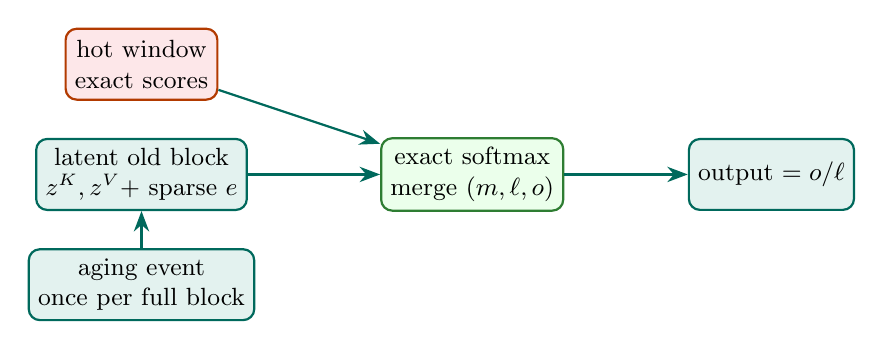
\begin{tikzpicture}[
  box/.style={draw=accent, fill=coolc, rounded corners, minimum height=0.9cm, align=center, thick, font=\small},
  hotb/.style={draw=accent3, fill=hotc, rounded corners, minimum height=0.9cm, align=center, thick, font=\small},
  mrg/.style={draw=accent2, fill=green!8, rounded corners, minimum height=0.9cm, align=center, thick, font=\small},
  ar/.style={-{Stealth[length=2.6mm]}, thick, accent},
  lab/.style={font=\scriptsize, text=accent!70!black}
]
\node[hotb] (hot) at (0,1.1) {hot window\\exact scores};
\node[box] (old) at (0,-0.3) {latent old block\\$z^K,z^V+$ sparse $e$};
\node[box] (age) at (0,-1.7) {aging event\\once per full block};
\node[mrg] (merge) at (4.2,-0.3) {exact softmax\\merge $(m,\ell,o)$};
\node[box] (out) at (8.0,-0.3) {output $=o/\ell$};
\draw[ar] (hot) -- (merge);
\draw[ar] (old) -- (merge);
\draw[ar] (age) -- (old);
\draw[ar] (merge) -- (out);
\end{tikzpicture}
\end{center}

% ================================================================
\section{Theory targets}

\begin{theorybox}
\textbf{(T1) Exactness of the merge.} The segmented softmax merge (Component~4) is
\emph{exact for the supplied block scores}: the only approximation is the latent$+$sparse KV
representation, isolated to the compressed segment's scores $s_{jt}$ and output $o_j$.
\end{theorybox}

\begin{theorybox}
\textbf{(T2) Attention-relevant error bound.} Bound the attention-output error
$\norm{\hat o/\hat\ell - o/\ell}$ in terms of (i) the residual KV energy after rank-$r$ $+$
$k$-sparse and (ii) the \emph{missed attention mass}, rather than the raw reconstruction error
$\norm{K-\hat K}$. This is the useful result: it ties tolerable compression to what attention
actually weights, so aggressive compression is safe exactly where attention mass is negligible.
\end{theorybox}

\begin{claim}[no-shuffle guarantee]
For every request admitted by Component~5 with prompt length plus
\texttt{max\_new\_tokens} at most $L$, Shufflerless-CI performs no large KV transfer during
steady-state decoding and the measured per-stage peak resident memory does not exceed $M_i$,
provided the implementation respects the reserved workspace. This is a deterministic
admission-control claim, not a probabilistic prediction claim.
\end{claim}

\begin{theorybox}
\textbf{(T3) Complexity crossover.} Characterize the $(r,k,W,B)$ regime in which Components
1--3, \emph{including} amortized aging, index/bitmap traffic, RoPE handling, and kernel-launch
overhead, are faster than dense attention or paging. This prevents memory compression alone
from being reported as a latency win.
\end{theorybox}

% ================================================================
\section{Evaluation plan}

\subsection{Project ramp}
\begin{enumerate}[leftmargin=1.6em,itemsep=1pt]
\item Calibrate fixed projection factors and measure residual concentration per layer/head;
compare pre- and post-RoPE spectra, but do not run SVD during generation.
\item Implement the RAP-aligned plug-in route for one layer; add the decoupled-RoPE route
only after the first route passes the quality and latency gates.
\item Add block-wise top-$k$ residual extraction and a fused latent--residual attention kernel.
\item Measure the full crossover, including the once-per-block aging cost (T3).
\item Integrate one CI-Inf~\cite{poster} stage, then jointly optimize the layer partition
and layer/head budgets.
\item Enforce admission control and validate the no-shuffle claim with transfer/page-fault
traces rather than allocator statistics alone.
\end{enumerate}

\subsection{Testbed, baselines, metrics}
\term{Testbed:} the poster's 3$\times$ Jetson Orin Nano cluster~\cite{poster}, LLaMA-3.2-3B,
16/6/6 split, plus the partition selected by the new planner. \term{Baselines:} dense-KV
CI-Inf; single-device and three-device dense inference under the same precision and power mode;
Palu~\cite{palu}, Eigen Attention~\cite{eigenattention}, RAP~\cite{rap}, OjaKV~\cite{ojakv},
and STAR-KV~\cite{starkv}; paging~\cite{pagedattention}; and ScoutAttention~\cite{scoutattention}
where a fair Jetson port is possible. Report unavailable kernels/code as a limitation rather
than silently omitting the method. \term{Metrics:}
\begin{itemize}[leftmargin=1.5em,nosep]
\item explicit-copy bytes, migrated/page-faulted bytes, and synchronization time per token
(the headline target is zero large KV movement for admitted requests);
\item network bytes per token; maximum accelerator-resident memory;
\item time-to-first-token and P50/P95 token latency; energy per token;
\item maximum admitted context length before any shuffle, at batch sizes 1 and $>1$;
\item LongBench / RULER quality, and \emph{GSM8K / coding accuracy} --- because aggressive cache
approximation disproportionately harms chained reasoning, this is the key quality guard.
\end{itemize}

\subsection{Performance gates (targets, not promised results)}
\begin{itemize}[leftmargin=1.5em,itemsep=1pt]
\item \term{Representation gate:} at least $2\times$ KV reduction with at most one
percentage point average task degradation; otherwise stop before systems integration.
\item \term{Kernel gate:} at least $1.25\times$ attention speedup over dense attention
at a memory-bound context, after amortizing aging. If it fails, make context capacity and tail
latency---not mean token latency---the paper's primary result.
\item \term{System target:} $1.5\times$ end-to-end throughput or a $2$--$4\times$ longer
admitted context at matched quality, with lower P95 latency than paging. Short-context batch-1
decoding is a required negative control and may show no gain.
\end{itemize}

\begin{riskbox}
\textbf{(a)} RoPE handling can erase the low-rank speedup, as reported for Eigen Attention;
make RAP-aligned projection the plug-in fallback and treat decoupled RoPE as an ablation.
\textbf{(b)} Sparse residual indexing may be slower than dense math; use block sparsity and
the kernel gate, falling back to latent-only or dense per layer.
\textbf{(c)} The fixed subspace may fail under prompt shift; increase the innovation budget
or keep sensitive heads exact rather than updating a basis online.
\textbf{(d)} Jetson unified memory can make ``CPU--GPU bytes'' ambiguous; trace migrations,
copies, faults, stalls, and memory-controller traffic separately.
\end{riskbox}

\begin{claimbox}
Shufflerless-CI is strongest as a \emph{systems co-design}, not as a new decomposition:
\emph{RoPE-safe latent birth for the stable bulk, block-wise sparse innovations for
input-specific error, and bottleneck-aware heterogeneous placement with deterministic
no-shuffle admission}. This version removes per-token SVD, remote per-layer KV calls, and an
RL controller from the critical path---the three choices most likely to erase performance.
\end{claimbox}

\subsection*{Reviewer-style verdict}
\textbf{Accept with revisions.} Faster has the highest ceiling (8/10) because the mechanism
removes cache transfer, dense reconstruction, and unnecessary online decomposition; Cheaper is
8/10 through longer contexts on fixed hardware; Stronger is 6/10 because sparse innovations
address prompt shift. Higher is 5/10 (quality preservation, not improvement) and Broader is 5/10.
The remaining major flaw is novelty proximity to Eigen Attention, RAP, OjaKV, LCA, and 2026 hybrid
KV methods. The defense is a decisive joint-optimization ablation: fixed partition plus the same
compressor versus joint representation/placement, with measured end-to-end gains. Feasibility is
yellow until the one-layer fused kernel passes the representation and kernel gates.

% ================================================================
\begin{thebibliography}{99}
\small
% --- base system / group ---
\bibitem{poster} H.~Zhou and X.~Zhang. \emph{Poster: Distributed Pipelined Collaborative Inference for LLMs on Edge Device Clusters.} ACM HotMobile 2026.
\bibitem{hexgen} Y.~Jiang et al. \emph{HexGen: Generative Inference of Large Language Model over Heterogeneous Environment.} ICML 2024. arXiv:2311.11514.
\bibitem{jupiter} S.~Ye et al. \emph{Jupiter: Fast and Resource-Efficient Collaborative Inference of Generative LLMs on Edge Devices.} IEEE INFOCOM 2025. arXiv:2504.08242.
\bibitem{foci} H.~Zhou and X.~Zhang. \emph{Fairness-Oracular MARL with Competitor-Aware Signals for Collaborative Inference.} NeurIPS 2025 Workshop (AI4NextG).
\bibitem{baq} L.~Zu, H.~Zhou, X.~Zhang. \emph{Behavior-Adaptive Q-Learning: A Unifying Framework for Offline-to-Online RL.} arXiv:2511.03695, 2025.
\bibitem{dare} L.~Zu, Y.~Qian, S.~Chakraborty, X.~Zhang. \emph{From Static Constraints to Dynamic Adaptation: Sample-Level Constraint Relaxation for Offline-to-Online RL (DARE).} ICML 2026. arXiv:2511.03828.
% --- KV compression (novelty boundary) ---
\bibitem{shadowkv} H.~Sun et al. \emph{ShadowKV: KV Cache in Shadows for High-Throughput Long-Context LLM Inference.} ICML 2025 (PMLR v267). arXiv:2410.21465.
\bibitem{lexico} J.~Kim, J.~Park, J.~Cho, D.~Papailiopoulos. \emph{Lexico: Extreme KV Cache Compression via Sparse Coding over Universal Dictionaries.} ICML 2025 (PMLR v267). arXiv:2412.08890.
\bibitem{gear} H.~Kang, Q.~Zhang, G.~Jeong, T.~Krishna, T.~Zhao. \emph{GEAR: An Efficient Error Reduction Framework for KV Cache Compression in LLM Inference.} PMLR v262, 2024. arXiv:2403.05527.
\bibitem{rocketkv} P.~Behnam et al. \emph{RocketKV: Accelerating Long-Context LLM Inference via Two-Stage KV Cache Compression.} ICML 2025 (PMLR v267). arXiv:2502.14051.
\bibitem{cake} S.~Jin et al. \emph{Compute Or Load KV Cache? Why Not Both? (CAKE).} ICML 2025 (PMLR v267). arXiv:2410.03065.
\bibitem{eigenattention} U.~Saxena, G.~Saha, S.~Choudhary, K.~Roy. \emph{Eigen Attention: Attention in Low-Rank Space for KV Cache Compression.} Findings of EMNLP 2024.
\bibitem{rap} J.~Xin et al. \emph{RAP: KV-Cache Compression via RoPE-Aligned Pruning.} arXiv:2602.02599, 2026.
\bibitem{ojakv} Y.~Zhu et al. \emph{OjaKV: Context-Aware Online Low-Rank KV Cache Compression.} Findings of ACL 2026.
\bibitem{starkv} P.~Bhatnagar et al. \emph{STAR-KV: Low-Rank KV Cache Compression via Soft Thresholding for Adaptive Rank Control.} arXiv:2606.08382, 2026.
\bibitem{lca} \emph{Latent-Condensed Transformer for Efficient Long Context Modeling.} ACL 2026.
\bibitem{mha2mla} Y.~Ji et al. \emph{Towards Economical Inference: Enabling DeepSeek's Multi-Head Latent Attention in Any Transformer-based LLMs.} ACL 2025.
\bibitem{deepseekv2} DeepSeek-AI. \emph{DeepSeek-V2: A Strong, Economical, and Efficient Mixture-of-Experts Language Model.} arXiv:2405.04434, 2024.
% --- distributed / collaborative attention ---
\bibitem{onlinesoftmax} M.~Milakov, N.~Gimelshein. \emph{Online Normalizer Calculation for Softmax.} arXiv:1805.02867, 2018.
\bibitem{flashattention} T.~Dao, D.~Y.~Fu, S.~Ermon, A.~Rudra, C.~R\'e. \emph{FlashAttention: Fast and Memory-Efficient Exact Attention with IO-Awareness.} NeurIPS 2022. arXiv:2205.14135.
\bibitem{ringattention} H.~Liu, M.~Zaharia, P.~Abbeel. \emph{Ring Attention with Blockwise Transformers for Near-Infinite Context.} NeurIPS 2023. arXiv:2310.01889.
\bibitem{scoutattention} \emph{ScoutAttention: Efficient KV Cache Offloading via Layer-Ahead CPU Pre-computation for LLM Inference.} DAC 2026. arXiv:2603.27138.
\bibitem{pagedattention} W.~Kwon et al. \emph{Efficient Memory Management for Large Language Model Serving with PagedAttention (vLLM).} SOSP 2023. arXiv:2309.06180.
% --- tensor / low-rank + sparse foundations ---
\bibitem{rpca} E.~J.~Cand\`es, X.~Li, Y.~Ma, J.~Wright. \emph{Robust Principal Component Analysis?} J.~ACM 58(3):11, 2011.
\bibitem{kolda} T.~G.~Kolda, B.~W.~Bader. \emph{Tensor Decompositions and Applications.} SIAM Review 51(3):455--500, 2009.
\bibitem{tt} I.~V.~Oseledets. \emph{Tensor-Train Decomposition.} SIAM J.~Sci.~Comput. 33(5):2295--2317, 2011.
\bibitem{losparse} Y.~Li et al. \emph{LoSparse: Structured Compression of Large Language Models based on Low-Rank and Sparse Approximation.} ICML 2023. arXiv:2306.11222.
\bibitem{linformer} S.~Wang, B.~Z.~Li, M.~Khabsa, H.~Fang, H.~Ma. \emph{Linformer: Self-Attention with Linear Complexity.} arXiv:2006.04768, 2020.
\bibitem{h2o} Z.~Zhang et al. \emph{H2O: Heavy-Hitter Oracle for Efficient Generative Inference of Large Language Models.} NeurIPS 2023. arXiv:2306.14048.
\bibitem{palu} J.~Chang et al. \emph{Palu: Compressing KV-Cache with Low-Rank Projection.} ICLR 2025. arXiv:2407.21118.
\end{thebibliography}

\end{document}
